\section{Introduction}

When modeling high-dimensional data where the number of features~(\(p\)) exceeds the number
of observations~(\(n\)), it is impossible to apply classical statistical models such as
standard linear regression since the design matrix \(\mat X\) is no longer of full rank. A
common remedy to this problem is to \emph{regularize} the model by adding a penalty term to
the objective that punishes models with large coefficients. The resulting problem takes the
following form:
\begin{equation}
  \label{eq:general-objective}
  \operatorname*{minimize}_{\beta_0 \in \mathbb{R},\vec{\beta} \in \mathbb{R}^p} g(\beta_0, \vec\beta; \mat X, \vec y) + h(\vec\beta),
\end{equation}
%
where \(g\) is a data-fitting function that attempts to optimize the fit to the data and
\(h\) is a penalty that depends only on \(\bm{\beta}\). Two common penalties are the
\(\ell_1\) norm and squared \(\ell_2\) norm penalties, which if \(g\) is the standard
ordinary least-squares objective, represent the
lasso~\citep{tibshirani1996,santosa1986,donoho1994} and ridge (Tikhonov) regression
respectively.

These penalties depend on the magnitudes of the coefficients, which means that they are
sensitive to the scales of the features in \(\mat X\). To avoid this, it is common to
\emph{normalize} the features before fitting the model by shifting and scaling each feature
by some measures of their locations and scales, respectively. For some problems it is
possible to arrive at these measure by contextual knowledge of the data at hand. In most
cases, however, they must be estimated. A popular strategy is to use the mean and standard
deviation of each feature as location and scale factors respectively, which is called
\emph{standardization}.

The choice of normalization may, however, have consequences for the estimated model. As a
first example of this, consider \Cref{fig:realdata-paths}, which displays the lasso paths
for two data sets and two types of normalization. Note that the choice of normalization
result in different sets of features being selected as well as different coefficient
estimates.

\begin{figure}[bpt]
  \centering
  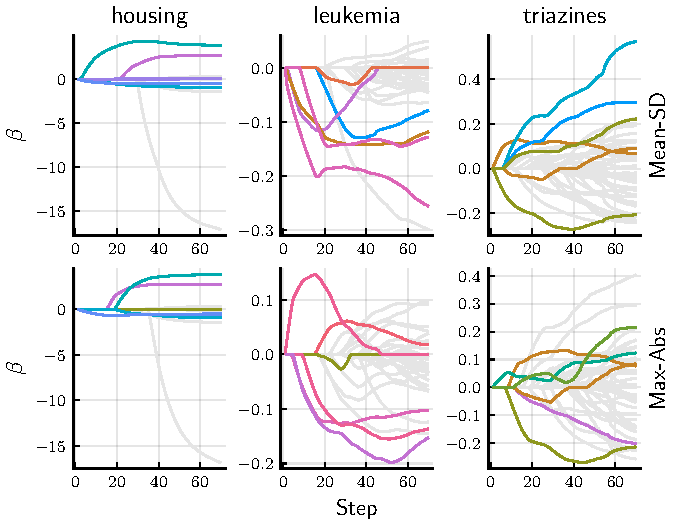
\includegraphics[]{realdata_paths.pdf}
  \caption{%
    Lasso paths for real datasets using two types of normalization:
    standardization and maximum absolute value normalization (max--abs). We have fit
    the lasso path to two four different datasets:
    \data{housing}~\citep{harrison1978}, \data{leukemia}~\citep{golub1999},
    \data{triazines}~\citep{king1995,hirst1994}, and \data{w1a}~\citep{platt1998}. (See \Cref{sec:data-summary}
    for more information about these data sets.) For each
    dataset, we have colored the coefficients if they were among the first five
    to become non-zero under either of the two normalization schemes.   }
  \label{fig:realdata-paths}
\end{figure}

In spite of this apparent connection between normalization and regularization, there has so
far been no research on the topic. And in its absence, the choice of normalization is
typically motivated by computational concerns or by being ``standard''. This is problematic
since the effects of normalization are unknown and because there exists no natural choice
for many types of data. In particular, there is no obvious choice for binary features
(where the each observations takes either of two values). In this paper we begin to bridge
this knowledge gap by studying normalization in the context of three particular cases of
\Cref{eq:general-objective}: the lasso, ridge, and elastic net~\citep{zou2005}. The latter
of these, the elastic net, is a generalization of the previous two, and is represented by
the following optimization problem:
%
\begin{equation}
  \label{eq:elastic-net}
  \operatorname*{minimize}_{\beta_0 \in \mathbb{R},\vec{\beta} \in \mathbb{R}^p} \frac{1}{2} \lVert \vec y - \beta_0 - \tilde{\mat{X}}\vec{\beta} \rVert^2_2  + \lambda_1 \lVert \vec\beta \rVert_1 + \frac{\lambda_2}{2}\lVert \vec \beta \rVert_2^2,
\end{equation}
%
where setting \(\lambda_1 = 0\) results in ridge regression and setting \(\lambda_2 = 0\)
results in the lasso. Our focus in this paper is on binary data and we pay particular
attention to the case when they are imbalanced, that is, have relatively many ones or
zeroes. In this scenario, we demonstrate that the choice of normalization directly
influences the regression coefficients and that this effect depends on the particular
combination of normalization and regularization. Our key contributions are:
\begin{enumerate}
  \item We reveal that class balance in binary features significantly affects lasso, ridge, and
        elastic net estimates, and show that scaling binary features with standard deviation
        (ridge) or variance (lasso) mitigates these effects at the cost of increased
        variance~(\Cref{sec:theory-binary-features}).
  \item For mixed data designs, we demonstrate that normalization choice implicitly determines how
        regularization affects binary versus continuous features~(\Cref{sec:mixed-data}).
  \item For interaction features, we provide guidelines on proper centering and scaling to mitigate
        class balance bias~(\Cref{sec:interactions}).
\end{enumerate}
